% Chapter 1

\chapter{Experiments and Results} % Main chapter title

\label{Chapter7_results} % For referencing the chapter elsewhere, use \ref{Chapter1} 

%----------------------------------------------------------------------------------------

% Define some commands to keep the formatting separated from the content 


%----------------------------------------------------------------------------------------



%\section{Experiments and Results}\label{sec:results}

In this section we present the evaluation of our algorithms. First we explain how the EV population is generated, and the time this generation process takes. Then, the performance of the algorithm is evaluated in terms of the quality of the formed coalition and also in terms of execution time and scaling behavior. All figures and tables present average values over multiple runs. Specifically, we generated $20$ hypergraphs  with $20,000$ EVs each, and then ran each algorithm on every hypergraph 10 times, and took the averages (and the average of those averages).
%First, we will see the time required to generate the pool of EVs we will be using in our tests. Next, we will present how each algorithm performed while it was running and when the coalitions were in the process of being formed. We will also test small modifications to our algorithms. Finally, we present graphs of how our algorithms scale with population and goals. 
%\subsection{A Note on Computational Requirements}
%Generation of the graph is $O(n)$. Each insertion is $O(1)$. For the minimal transversal algorithm the complexity as calculated in \cite{kavvadias2005efficient} is $O(\log^2 n)$. That's for calculating all the minimal transversal sets. For the heuristic approach, normal sorting complexity is applied on the pruned hypergraph.
Our experiments were run on a Sandy Bridge i7-2600K at 4.2 GHz. All the tests were running on a single thread on Python, meaning that there is a lot of room for optimization. %To generate the graphs below 20 sets of starting EVs were made for each pool size and the algorithms run ten times in each one. This was done to balance out the timing errors %that could be introduced from the different set of EVs. 

\begin{figure}\centering
	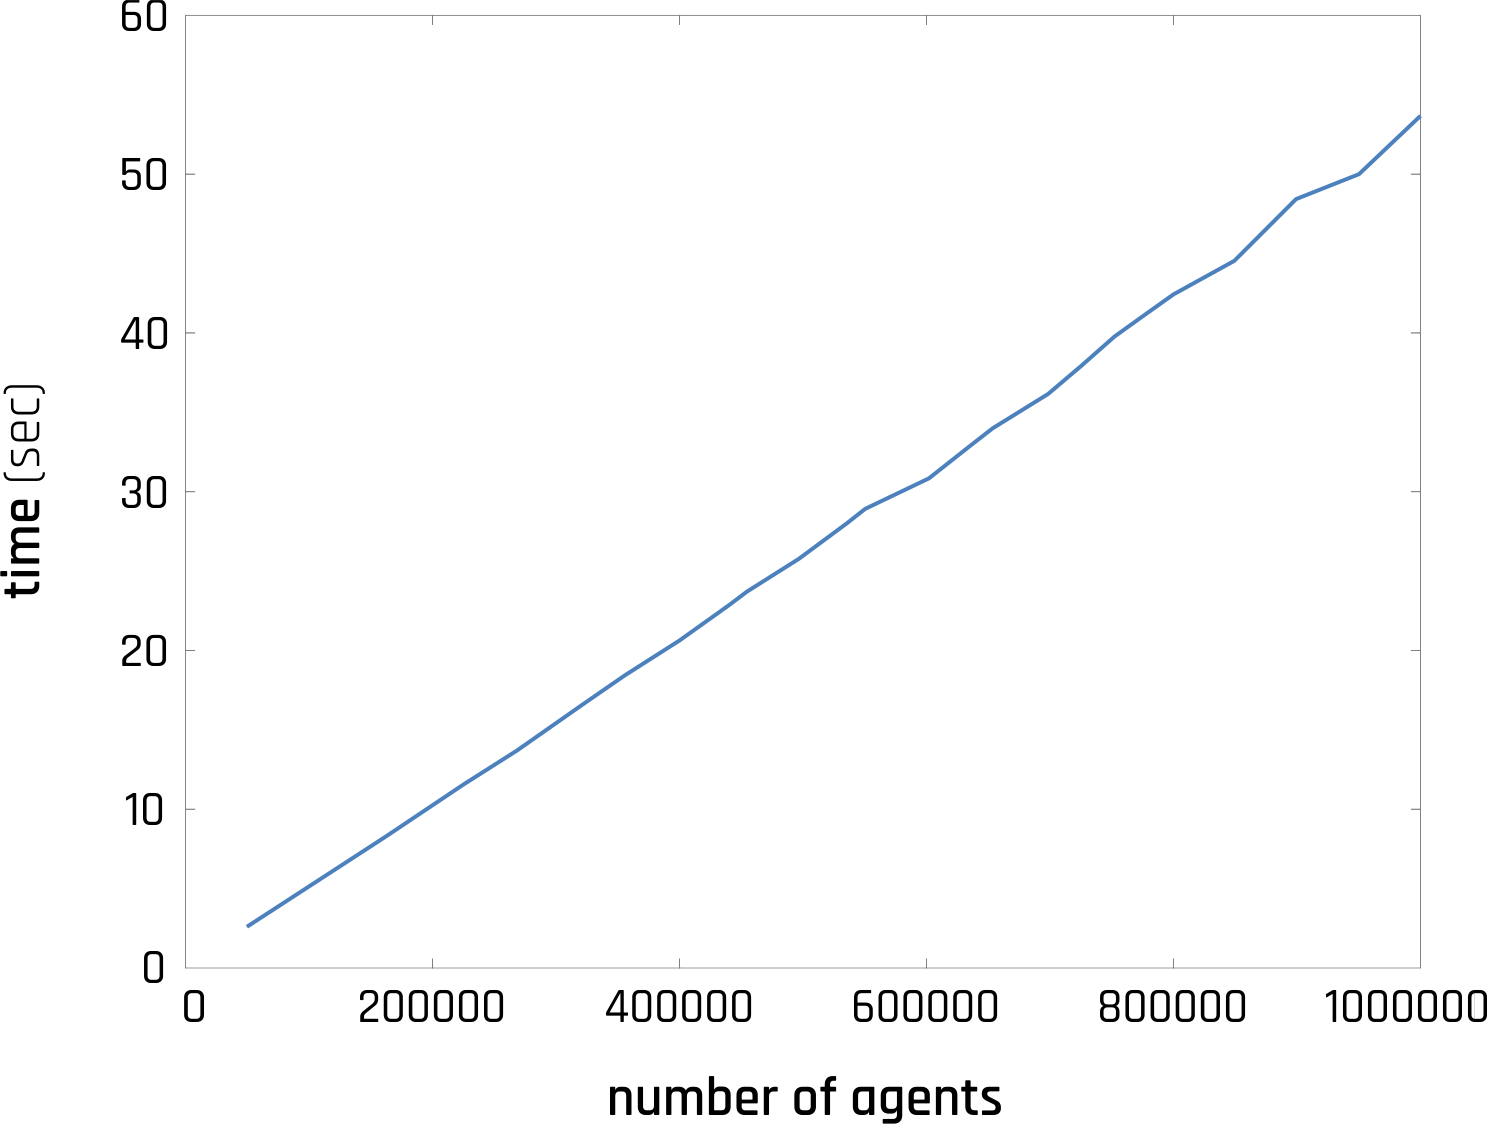
\includegraphics[scale=1]{generation_scaling.png}
	\vspace{10pt}
	\caption{Hypergraph generation scaling\label{fig:genscaling}}
\end{figure}

\section{Generating the EV Population}\label{sec:generating}
To generate the population for each type of experiment we create the vehicles one by one, by first generating its properties as follows. The capacity of each vehicle is generated from a Gaussian distribution with mean value $100$ and $\sigma = 80$. The discharge rate of each vehicle is generated from a Gaussian distribution with mean value $10$ and $\sigma=5$. The reliability of each vehicle is picked from a Gaussian distribution with mean value $0$ and $\sigma=1$. Each EV's commitment of being connected to the Grid is a {\em true} / {\em false} variable, with a $0.9$ probability of being {\em true}. If {\em true}, then the EV is inserted in the {\em committed} hyperedge. When a vehicle has its properties created, it is added in the pool of available EVs. The computational complexity of generating the hypergraph is, as expected, $O(n)$.

The coalition requirements are set to values which are commonly used in the regulation market \cite{kamboj2011deploying}, namely the following two. First, each coalition must have a total capacity of at least $10MWh$. The discharge rate must also be at least $1MW$ \cite{kamboj2011deploying}
These values are kept constant throughout all experiments---except when we test scaling against an increasing capacity goal, where capacity is treated as a variable.
\footnote{As stated in Chapter~\ref{Chapter6_approach}, our hypergraph used 25 hyperedges to store the attributes.}


Creating the hypergraph is a problem that scales linearly with time. Specifically, generating the hypergraph, including the vehicles and distributing them to hyperedges, takes a very small amount of time and scales linearly up to a million within a minute (Table ~\ref{tab:genscaling} and Fig~\ref{fig:genscaling}).
	\begin{table}
		\begin{center}
			\begin{tabular}{| c || c | }
				\hline
				EVs & Generation Time (sec) \\ \hline
				100,000  & 5.08\\ \hline
				200,000  & 10.23 \\ \hline
				300,000  & 15.31  \\ \hline
				400,000 & 20.51  \\ \hline
				500,000 & 25.75   \\ \hline
				600,000 & 30.69   \\ \hline
				700,000 & 36.14   \\ \hline
				800,000 & 42.38   \\ \hline
				900,000 & 48.37   \\ \hline
				1,000,000 & 53.62   \\ \hline
			\end{tabular}
		\end{center}    
		\caption{Hypergraph generation scaling timings\label{tab:genscaling}}
	\end{table}
\begin{table}
	\begin{center}
		\begin{tabular}{| c || c | c | }
			\hline
			Algorithm & Nodes after Pruning & Edges after Pruning \\ \hline
			Transversal & 1148.4   & 4  \\ \hline
			Clustering  & 1218.8   & 7 \\ \hline
			Heuristic   & 18012.6  & 25 \\ \hline
		\end{tabular}
	\end{center} 
	\caption{Pruning Results\label{tab:pruningres}}
\end{table}
As mentioned above, the initial EV population was $20,000$ nodes. However, before feeding the nodes to the algorithms, we pruned the hypergraph to keep promising nodes. Table~\ref{tab:pruningres} shows the average hypergraph size finally fed to the algorithms.

\section{Forming the Coalitions}
We now proceed to evaluate the performance of our algorithms. Our evaluation will examine {\em (a)} how fast and {\em (b)} by selecting how many vehicles they can meet the set requirements. Naturally, the faster an algorithm forms a coalition that meets all the requirements, the better. 
\begin{figure}
	\centering
		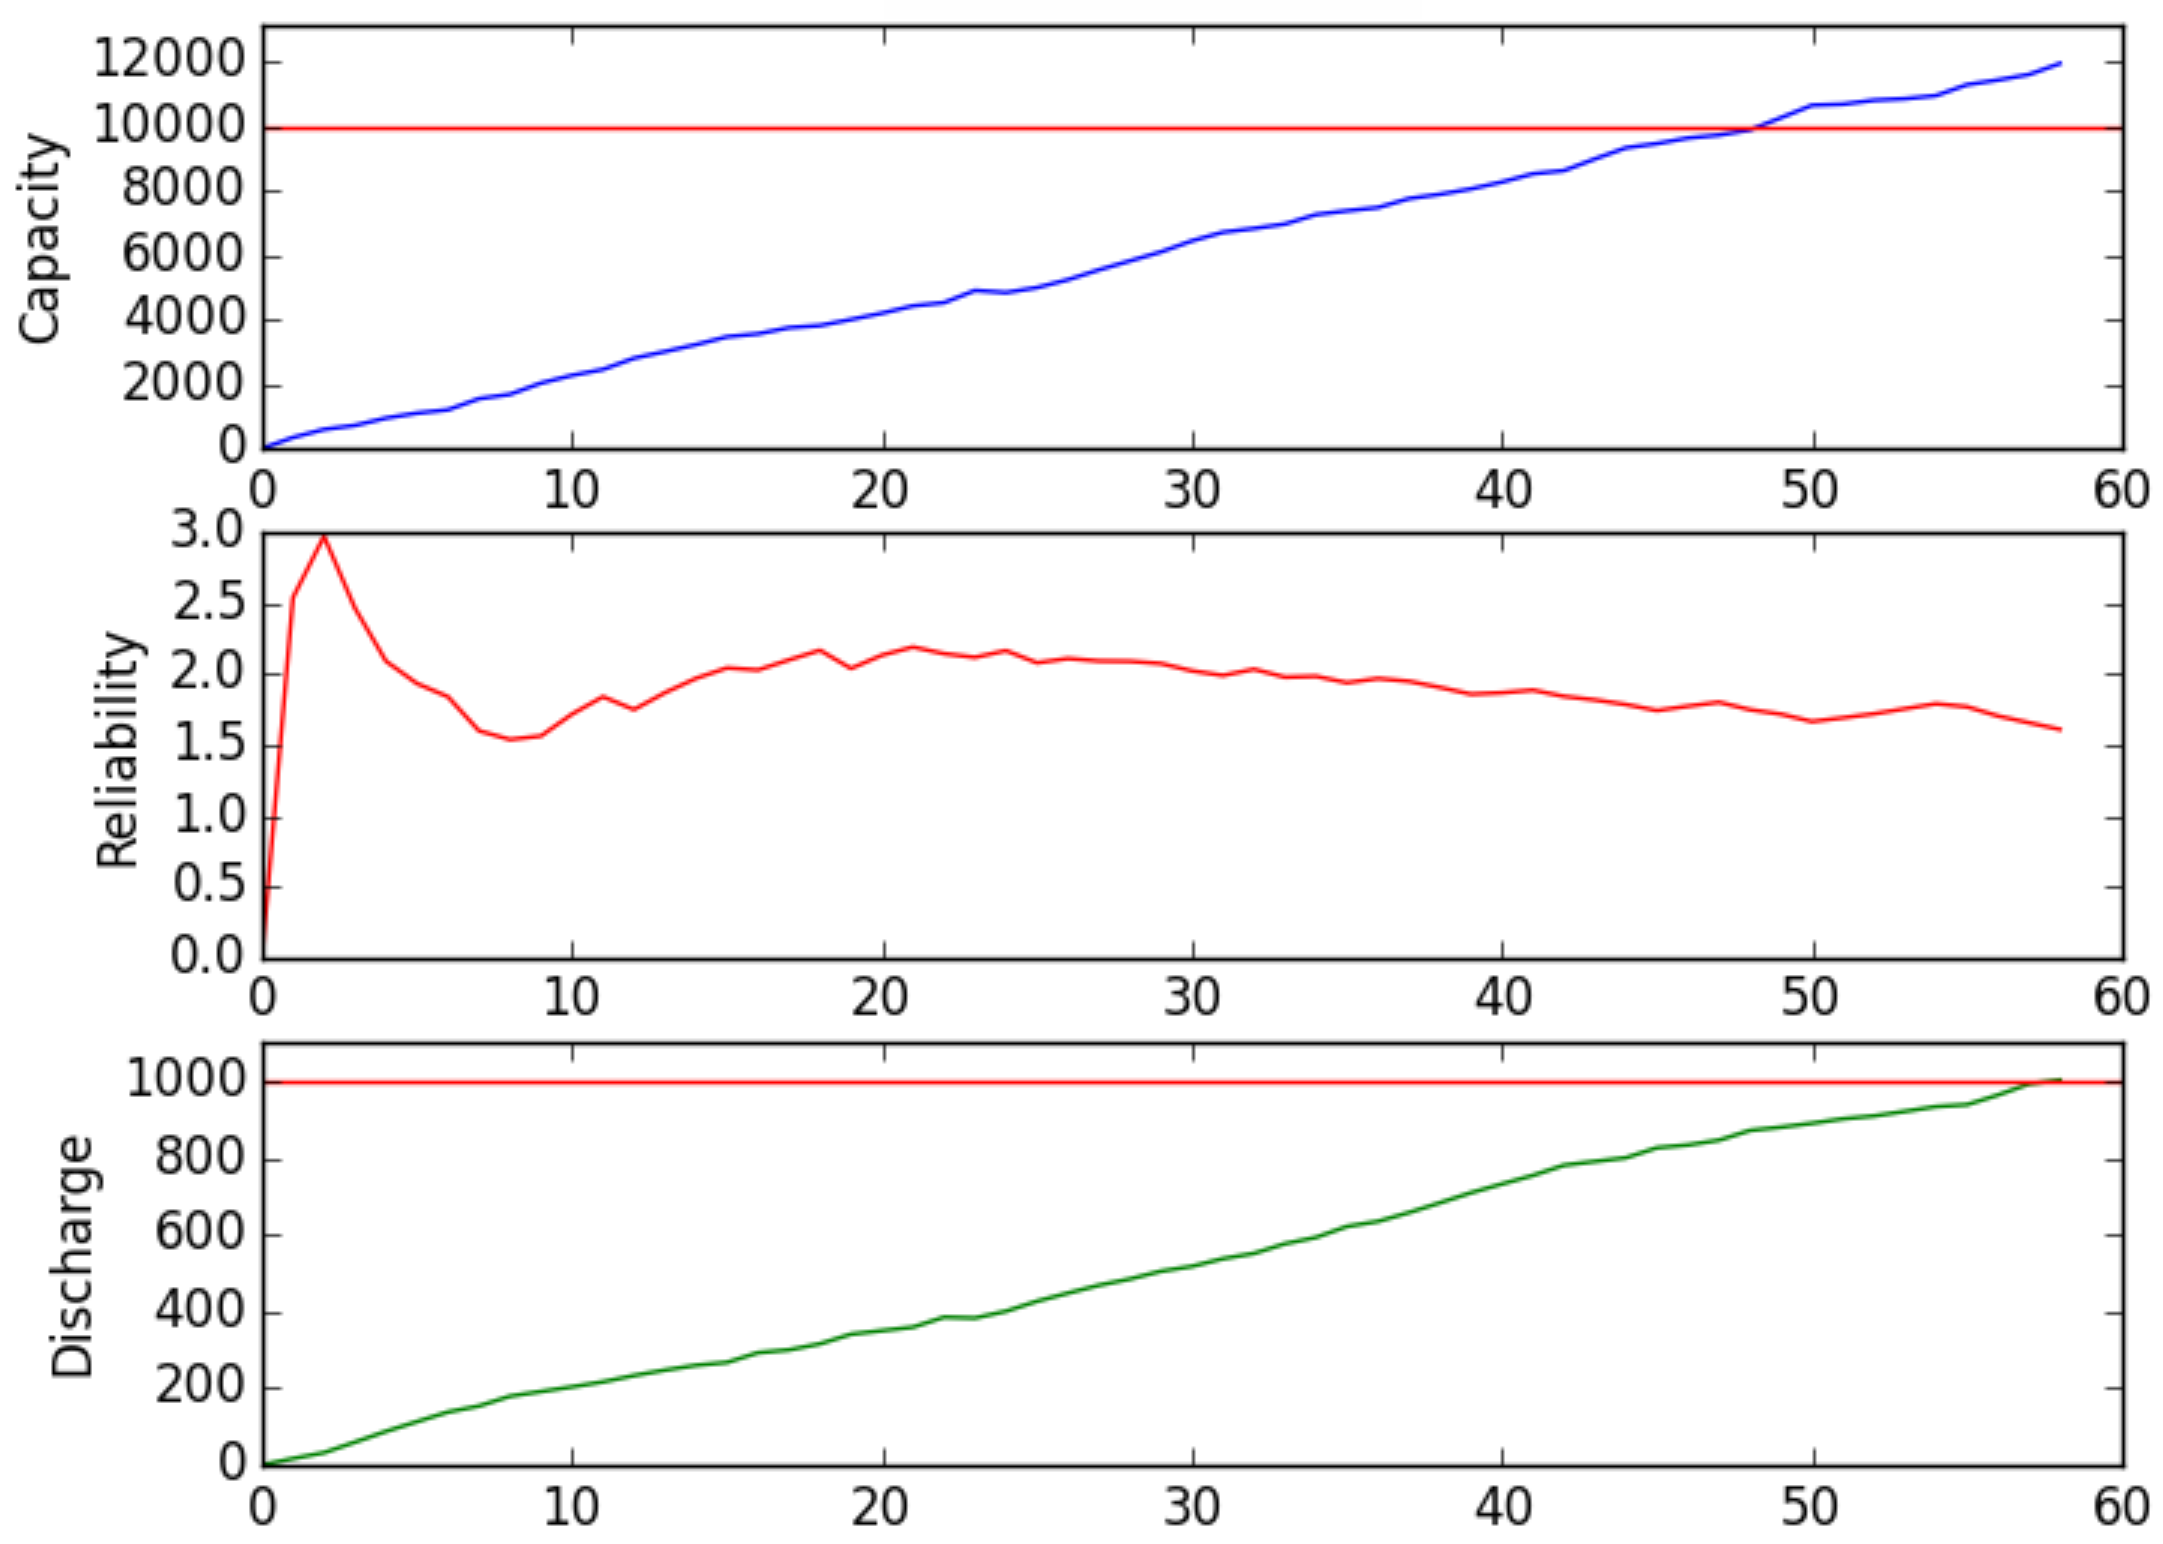
\includegraphics[scale=1]{greedy.png}
		\caption{Coalition formation with the\newline
			Heuristic Algorithm \label{fig:heuristiccoalcreate}}
\end{figure}
\begin{figure}	
	\centering
		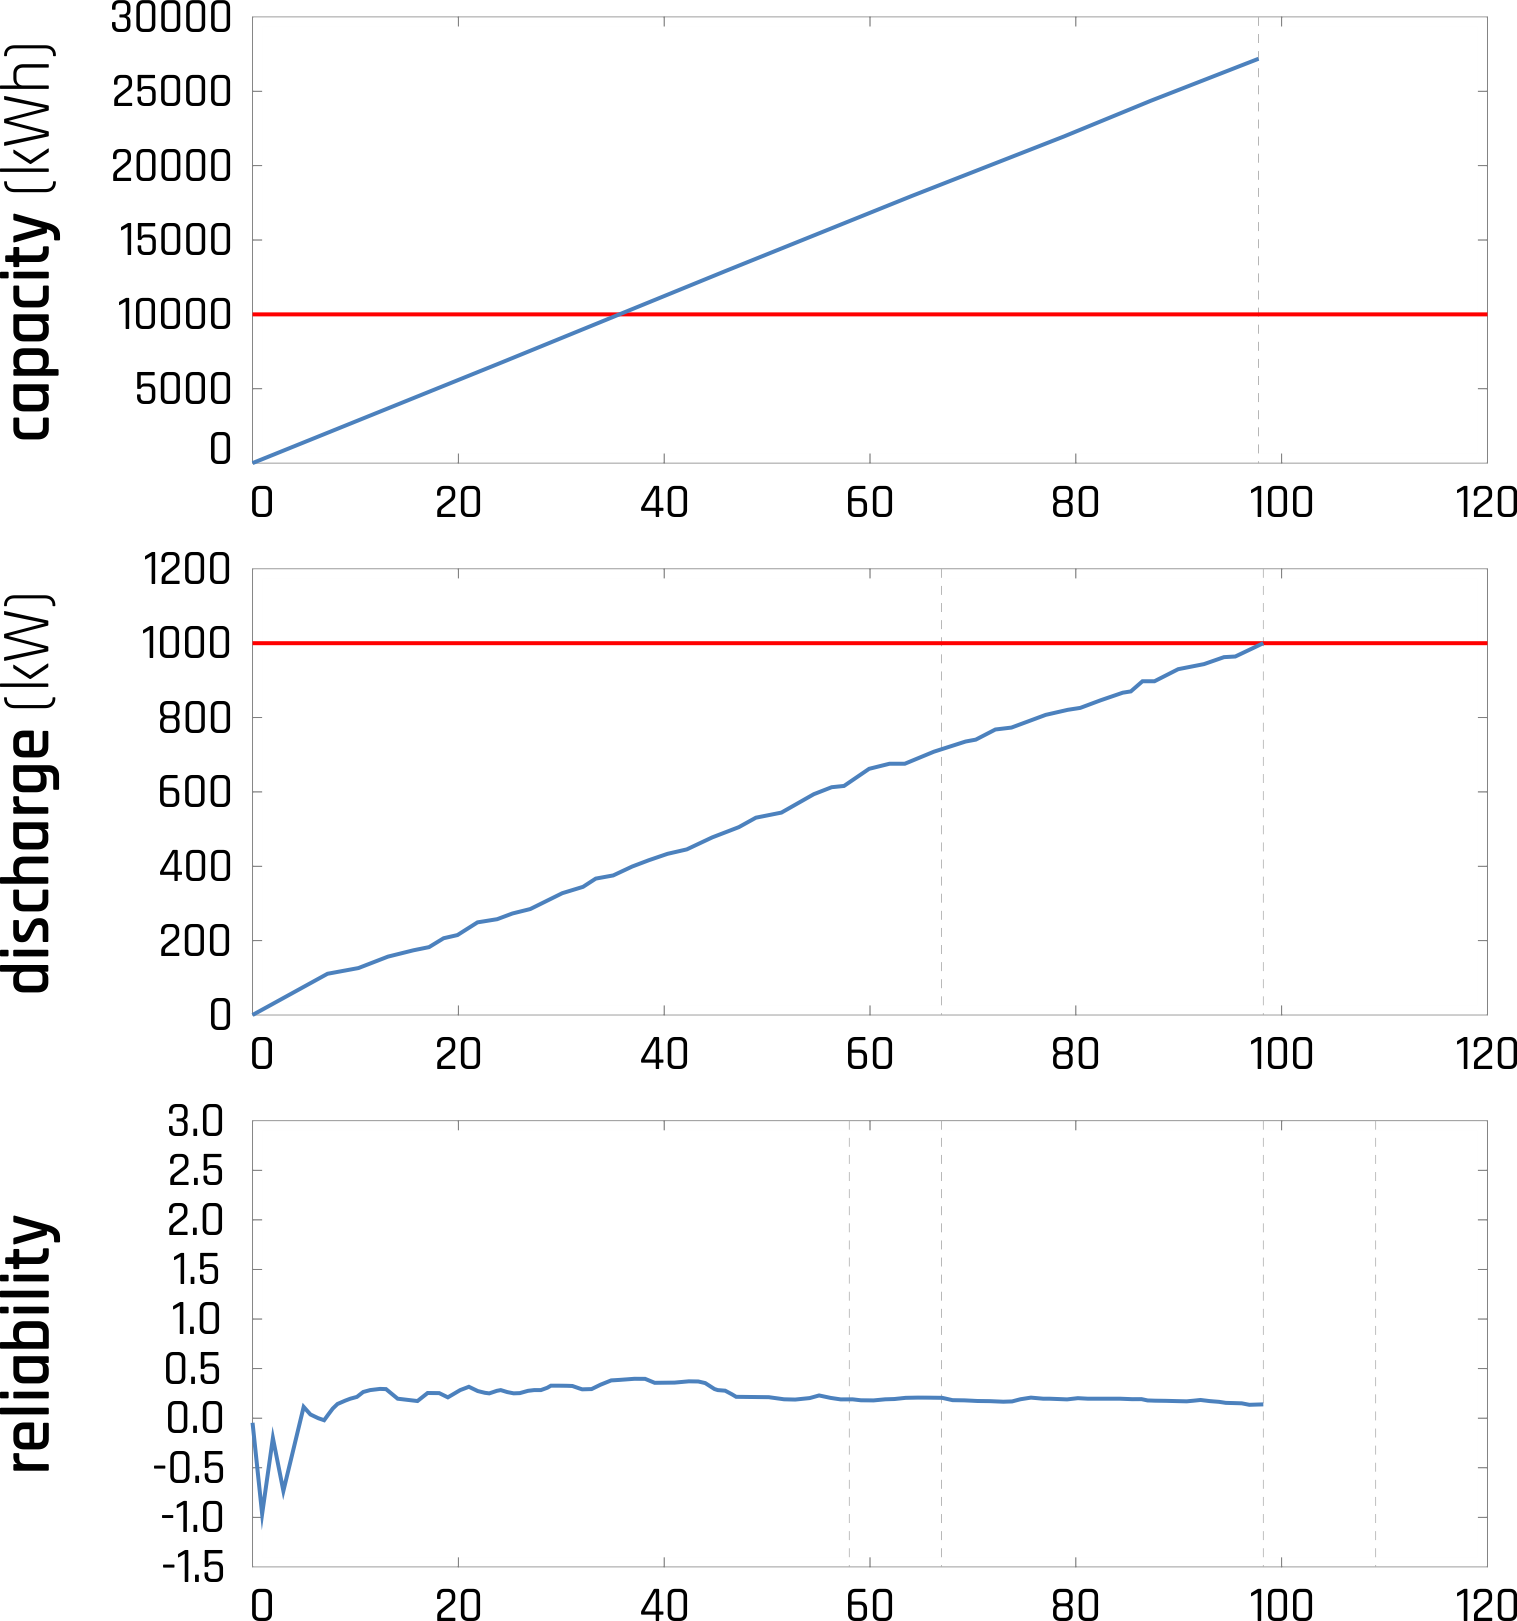
\includegraphics[scale=1]{clustering.png}
		\caption{Coalition formation with the\newline Clustering Algorithm\label{fig:clusteringcoalcreate}}
\end{figure}

Moreover, coalitions with fewer vehicles are preferable, since intuitively, this allows for a more efficient allocation of resources, and also means that fewer EVs will share the payoff associated with forming the coalition (exactly how this payoff allocation will occur, is a problem we do not deal with in this thesis).
%On the figures~\ref{fig:samplecoalcreate}-~\ref{fig:transversalcoalcreate} the following is displayed:

To begin, in all Figs.~\ref{fig:heuristiccoalcreate}---\ref{fig:samplecoalcreate}:
\begin{itemize}
	\item In all subfigures, the horizontal axis depicts the progression of the coalition size.
	\item {\em Capacity subfig.} On the first graph of each figure, the capacity of the coalition is displayed. We can see how it is increased by selecting the appropriate agents until the goal (horizontal line) is reached.
	\item {\em Reliability subfig.} The second graph displays the mean reliability of our coalition.
	\item {\em Discharge subfig.} The third and last graph displays the discharge rate of the coalition. The goal of $1,000$ kW is shown as a horizontal line.
\end{itemize}
%As mentioned above, the lower the average completion time and the lower average coalition, the better. 
\paragraph{Heuristic Algorithm}
As explained in Section~\ref{sec:heuristic}, this algorithm attempts (in a rather ``greedy'' manner) to identify the best EVs from the hypergraph.	As we can observe in Fig.~\ref{fig:heuristiccoalcreate}, it takes on average only $58.5$ vehicles to reach the goal requirements, which is the most efficient use of resources observed across all our methods. The reliability achieved is also high, reaching a value of more than $1.5$. We remind the reader that the mean reliability of our pool of EVs is $0$. This approach is also the most time and memory efficient of all. Specifically the algorithms average completion time is only $25ms$ for these experiments, and it also scales linearly into the millions as seen in Fig.~\ref{fig:heuristicscaling} below.	
\begin{figure}
	\centering
	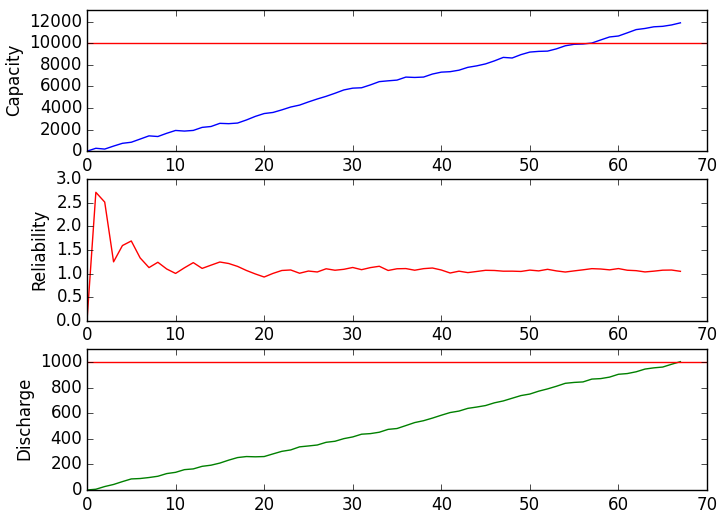
\includegraphics[scale=1]{transversal.png}
	\caption{Coalition formation with the\newline
		Minimal Transversal Algorithm \label{fig:transversalcoalcreate}}
\end{figure}
\paragraph{Clustering Algorithm}
This method performs clustering, as explained in Section~\ref{sec:Clustering}, and then takes random samples from the best cluster. Fig.~\ref{fig:clusteringcoalcreate} depicts its performance when using $k=3$ clusters. Unfortunately, we cannot control how exactly the clusters are formed, so we do not have a guarantee that high quality vehicles will be clustered together. This leads to a mediocre result with an increased average coalition size, and a slightly-over-the-average reliability. The average size of coalitions meeting both requirements is $98$. The average time required for the method's completion is $709 ms$. In Section~\ref{sec:results_modifications}, we show how different $k$ values affect our results.
\begin{figure}		
	\centering
		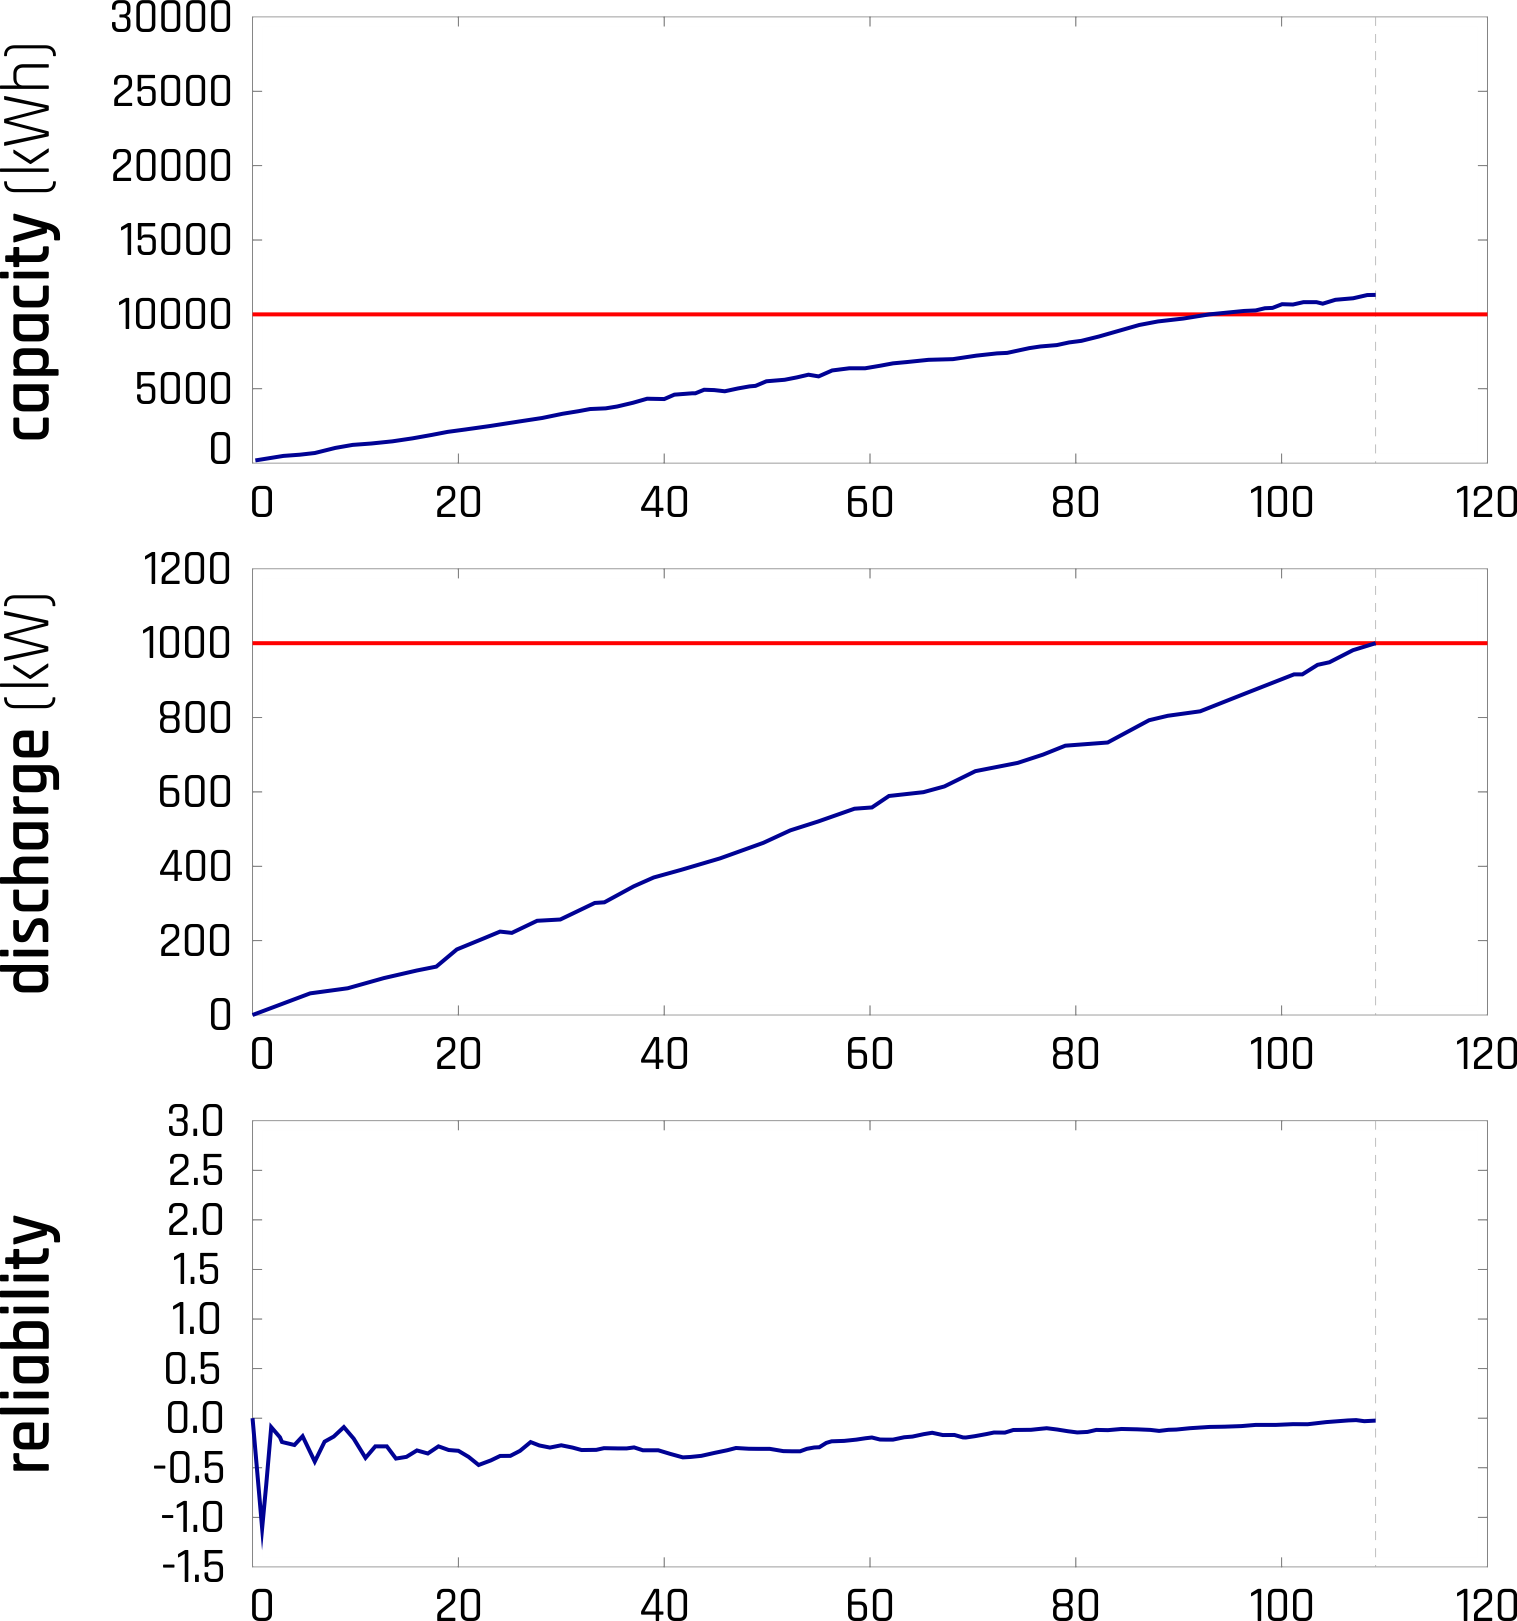
\includegraphics[scale=1]{sample.png}
		\caption{Coalition creation with the\newline
			Simple Sampling Algorithm \label{fig:samplecoalcreate}}
\end{figure}
\paragraph{Transversal}	
Using the transversal algorithm and taking nodes from a list of minimal hitting set. Fig.~\ref{fig:transversalcoalcreate} shows its performance. The transversal algorithm appears to work quite well since the average coalition size is only 64, slightly higher than that achieved by the heuristic approach. The reliability of the coalition is high, reaching  values over $1.1$. It can also scale quite well, reaching thousands of vehicles (cf. Fig.~\ref{fig:popscale} and Table~\ref{tab:popscale}), but not as well as the heuristic approach. The average time to completion was $120ms$. %only.
\begin{figure}		
	\centering
	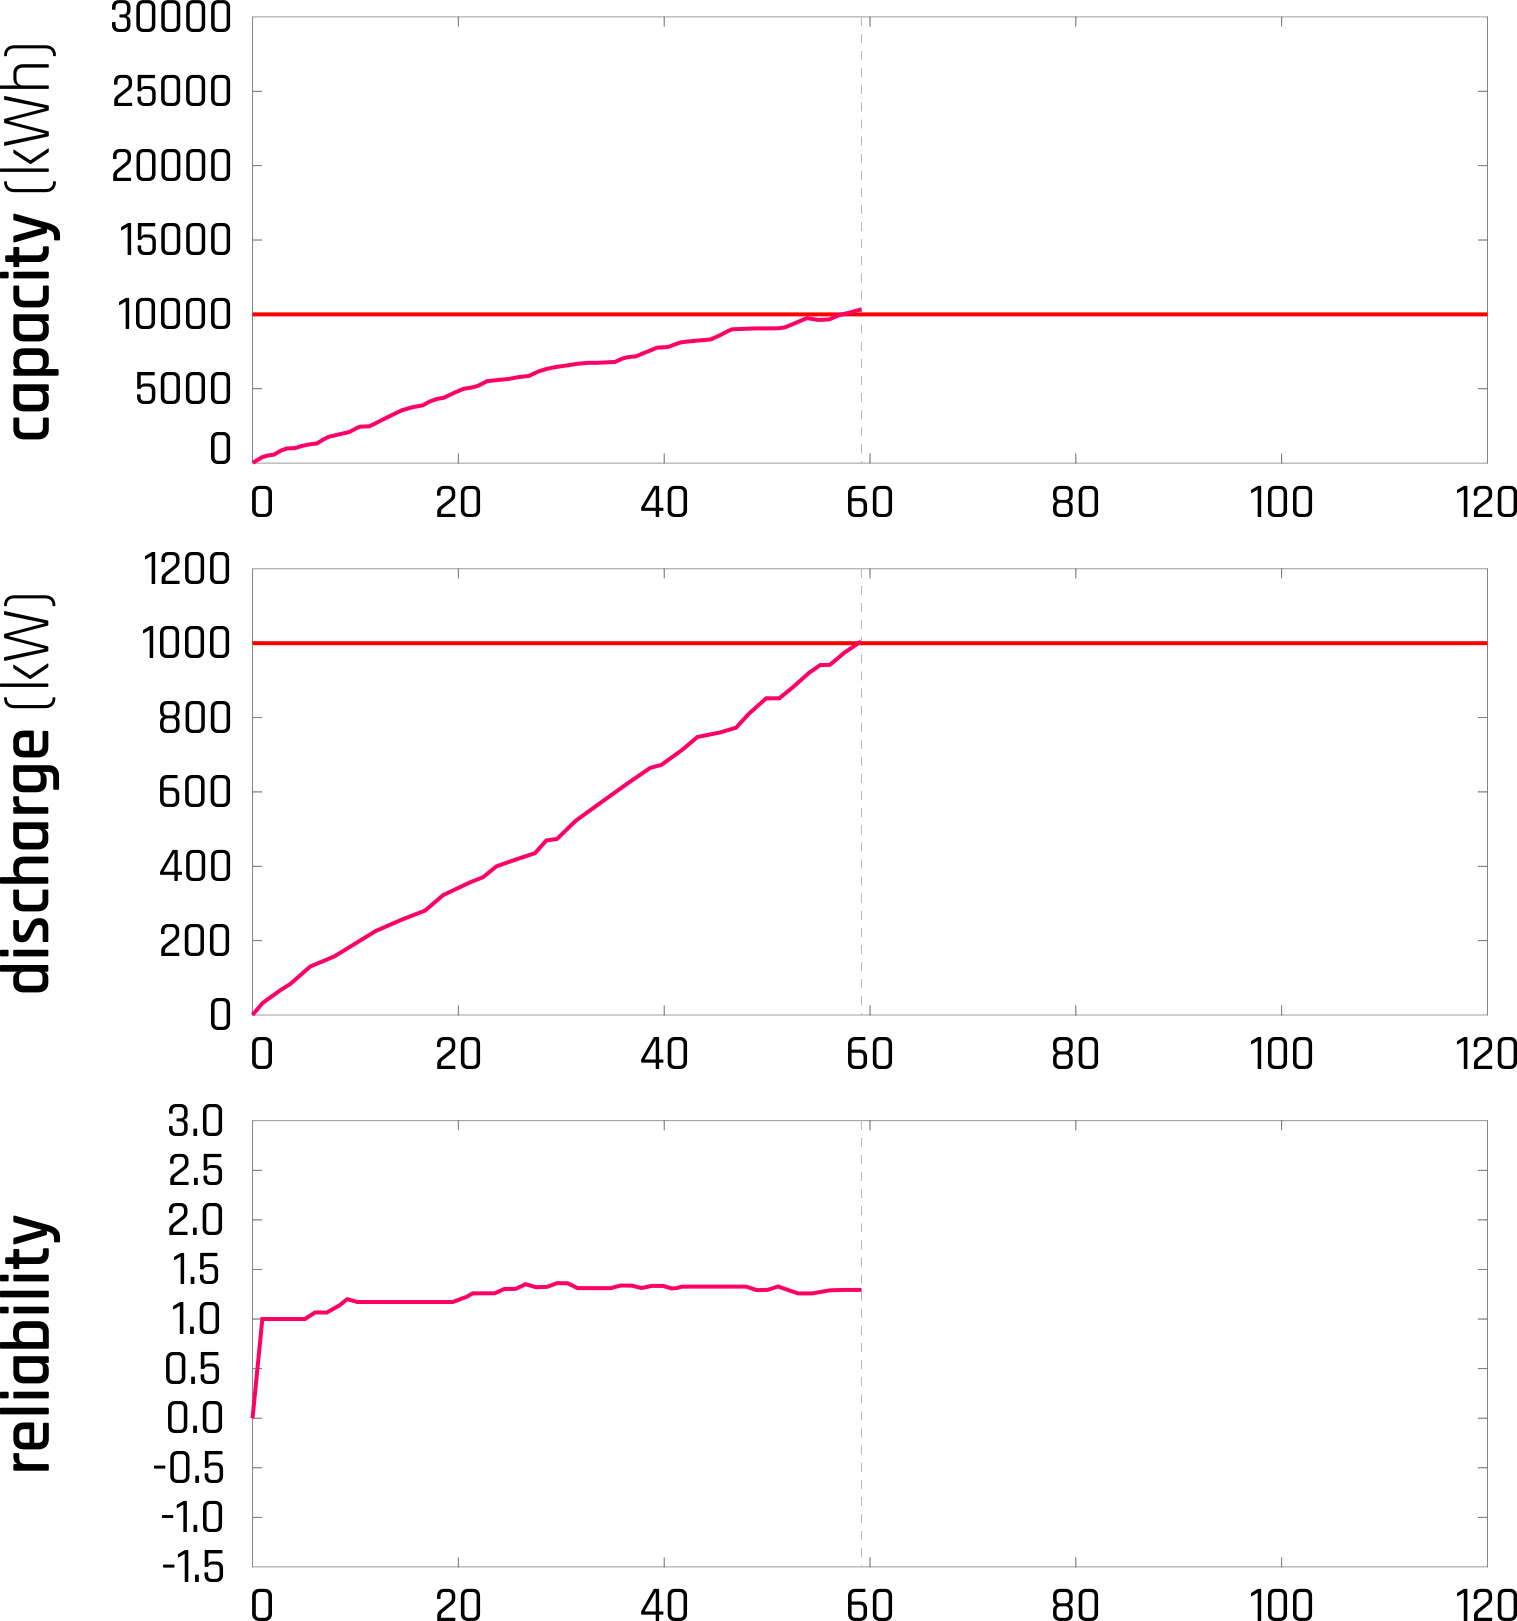
\includegraphics[scale=1]{hybrid.png}
	\caption{Coalition creation with the\newline
		Hybrid Algorithm \label{fig:hybridcoalcreate}}
\end{figure}
\paragraph{Hybrid}	
The hybrid algorithm takes EVs from coalitions created with transversal and heuristic. It runs faster than the transversal algorithm with better results while still having the advantages discussed in Sec.~\ref{sec:transversal}. Fig.~\ref{fig:hybridcoalcreate} depicts its performance. The average coalition size is just a bit higher than the heuristic at 59.6. Finally the mean running time is 75ms.



\paragraph{Simple Sampling}
%Taking random samples until the set capacity and discharge goals, are achieved. 
Fig.~\ref{fig:samplecoalcreate} depicts our results for the Simple Sampling method. The average coalition size achieved with this algorithm is 109.3. The average completion time was 24ms. As expected, this algorithm achieves the weakest results among all our algorithms.

Finally, Fig.~\ref{fig:coal_create_all} and Table~\ref{tab:resultssum} summarize the results for convenience. In the figure it can be easily seen that the hybrid and heuristic approach manage smaller coalitions by balancing correctly between {\em discharge} and {\em capacity} and finding overall good EVs. It can also be seen that the clustering algorithm selects high capacity EVs early on, thus wasting a lot of potential afterwards, by having to select the rest of the EVs to reach the {\em discharge} goal. This can be mitigated by increasing the number of clusters (Sec.~\ref{sec:results_modifications})

\begin{figure}		
	\centering
	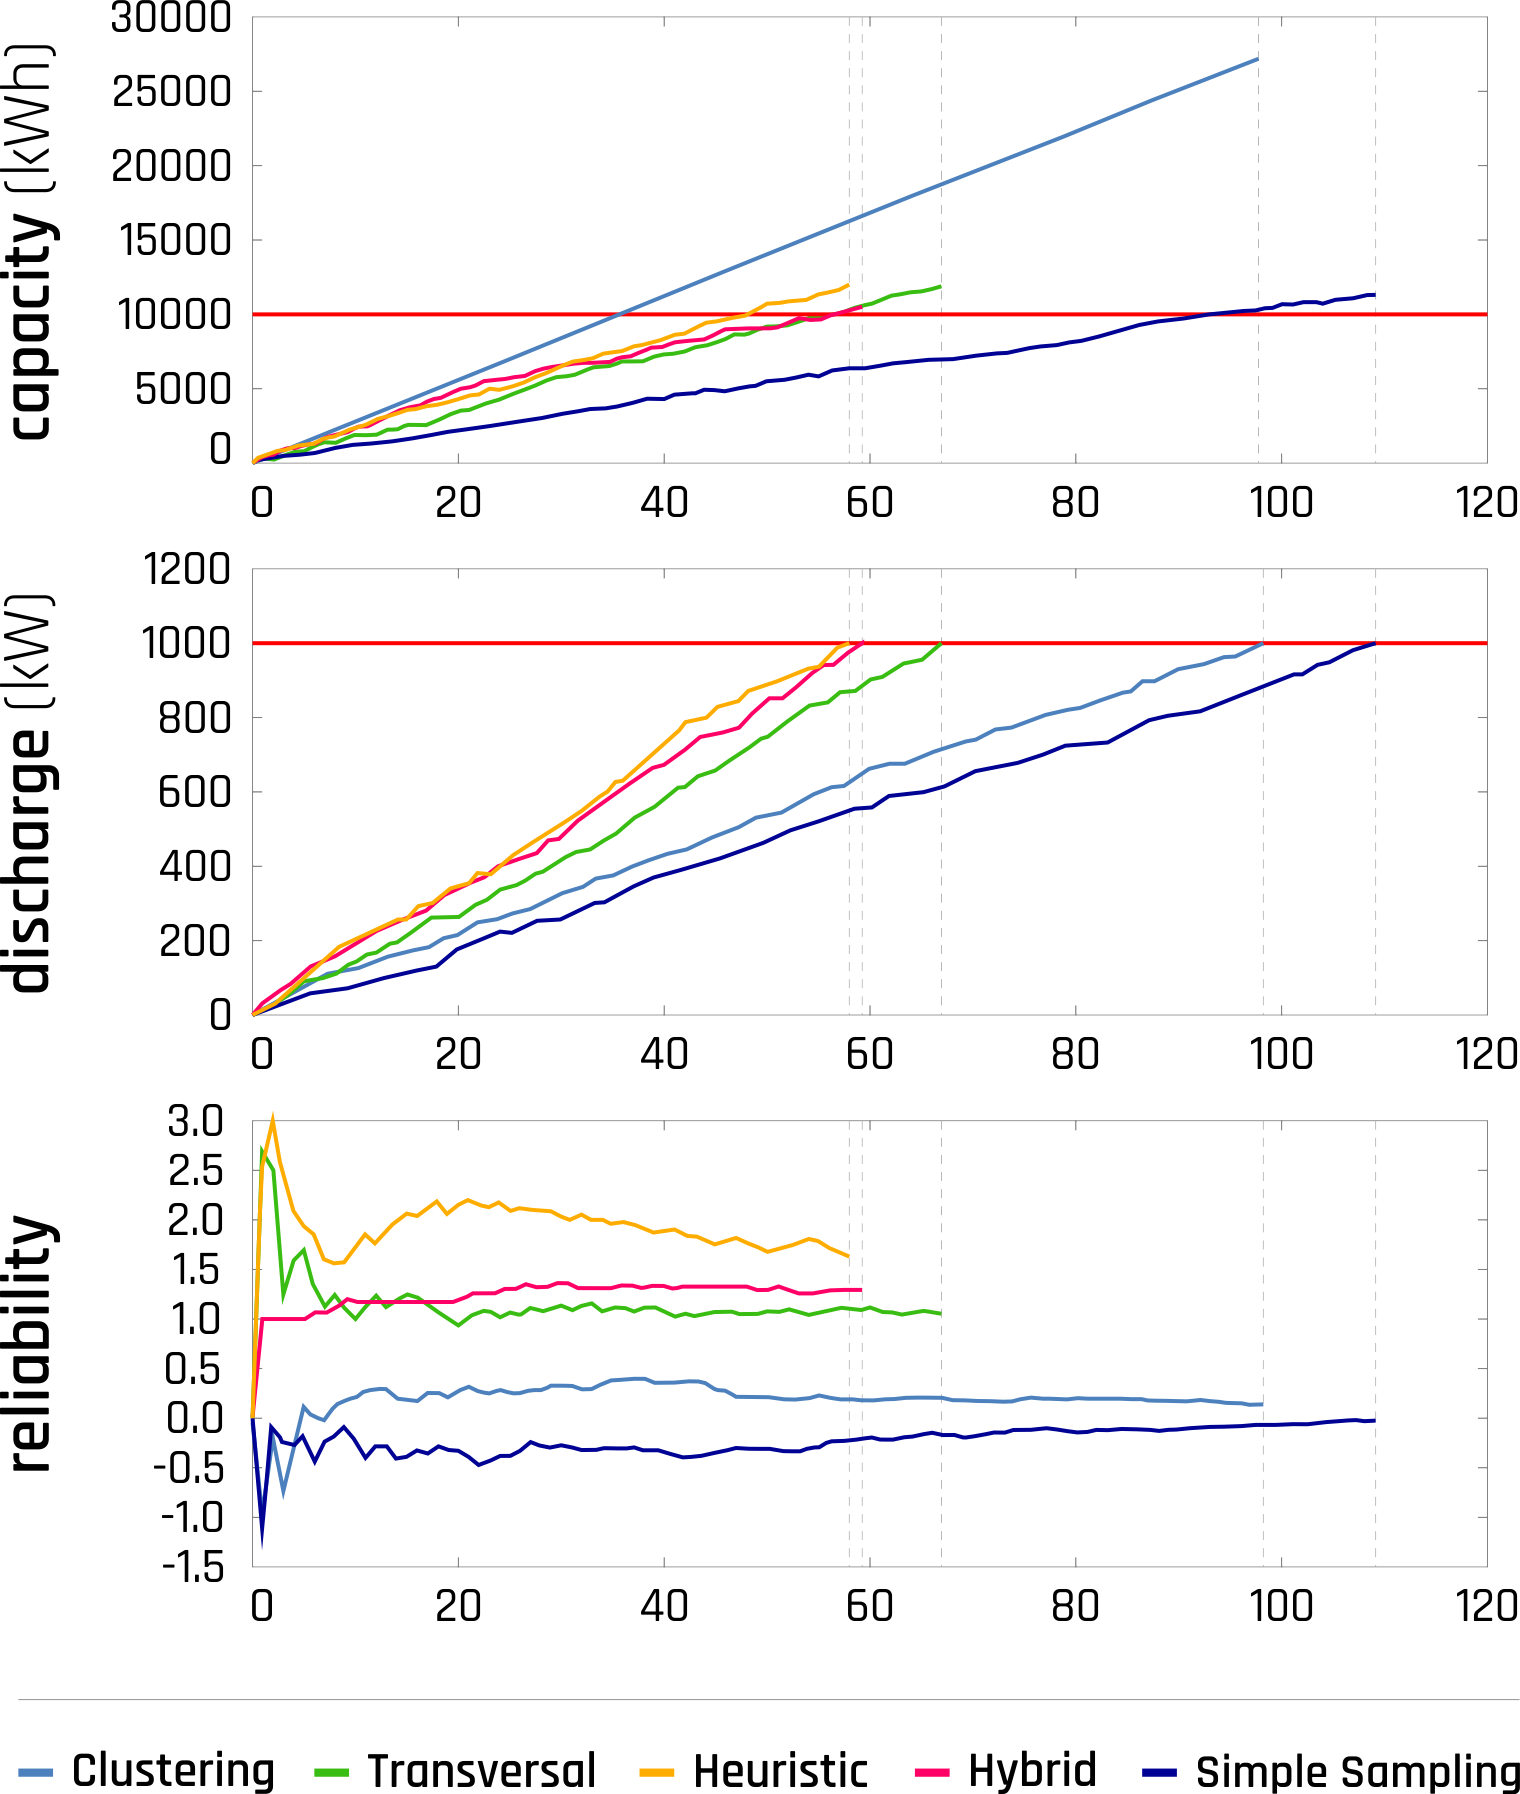
\includegraphics[scale=1]{coal_create_all.png}
	\caption{Coalition creation\label{fig:coal_create_all}}
\end{figure}

\begin{table}
	\begin{center}
		\begin{tabular}{| c || c | c | c | }
			\hline
			Algorithm  	& Coal. Size(\#EVs) & Run. Time($ms$) & Gen.+Run. Time($ms$)\\ \hline
			Heuristic	& 58.5 & 25 & 1041\\ \hline
			Clustering 	& 98 & 709 & 1725\\ \hline
			Transversal &  64 & 120  & 1136 \\ \hline
			Hybrid &  59.6 & 75  & 1091\\ \hline
			Sampling &  109.3 & 24  & 1040\\ \hline
		
		\end{tabular}
	\end{center}
	
	\caption{Summarizing the performance results\label{tab:resultssum}}
\end{table}	

\section{Scaling Behaviour}
We now test the scaling behaviour of our algorithms. First, we show how our algorithms scale with time when the \textit{capacity} goal is increased. Then, we show how they scale as the number of EVs  under consideration increases.

	\begin{table}
		\begin{center}
			\begin{tabular}{| c || c | c | c | }
				\hline
				Goal (kWh)& Heuristic (sec) & Clustering (sec) & Transversal (sec) \\ \hline
				10,000  & 0.03& 0.049 & 0.20\\ \hline
				40,000  & 0.04 & 0.049 & 0.36  \\ \hline
				70,000  & 0.06 & 0.049 & 0.34  \\ \hline
				100,000 & 0.11 & 0.049 & 0.33 \\ \hline
				130,000 & 0.19 & 0.049 & 0.33  \\ \hline
				160,000 & 0.28 & 0.049 & 0.33  \\ \hline
				190,000 & 0.39 & 0.049 & 0.34  \\ \hline
				220,000 & 0.50 & 0.049 & 0.32  \\ \hline
				250,000 & 0.64 & 0.049 & 0.32  \\ \hline
				280,000 & 0.86 & 0.049 & 0.32  \\ \hline
			\end{tabular}
		\end{center}
		\caption{Scaling against an increasing ``capacity'' goal\label{tab:goalscale}}
	\end{table}

In Fig.~\ref{fig:goalscale} and Table~\ref{tab:goalscale} 
we can see how the transversal, heuristic and clustering algorithm scale against an increasing capacity goal (assuming any other goal remains fixed). The starting size of the available agents was kept constant at $20,000$ EVs for this experiment. We observe that the scaling behaviour of the heuristic algorithm against an increasing capacity goal is exponential. %  in execution time. 
Nevertheless, its total required execution time is low, since it takes the algorithm 0.9 seconds to reach the goal capacity of 300,000 $kWh$.
\begin{figure}
	\centering
		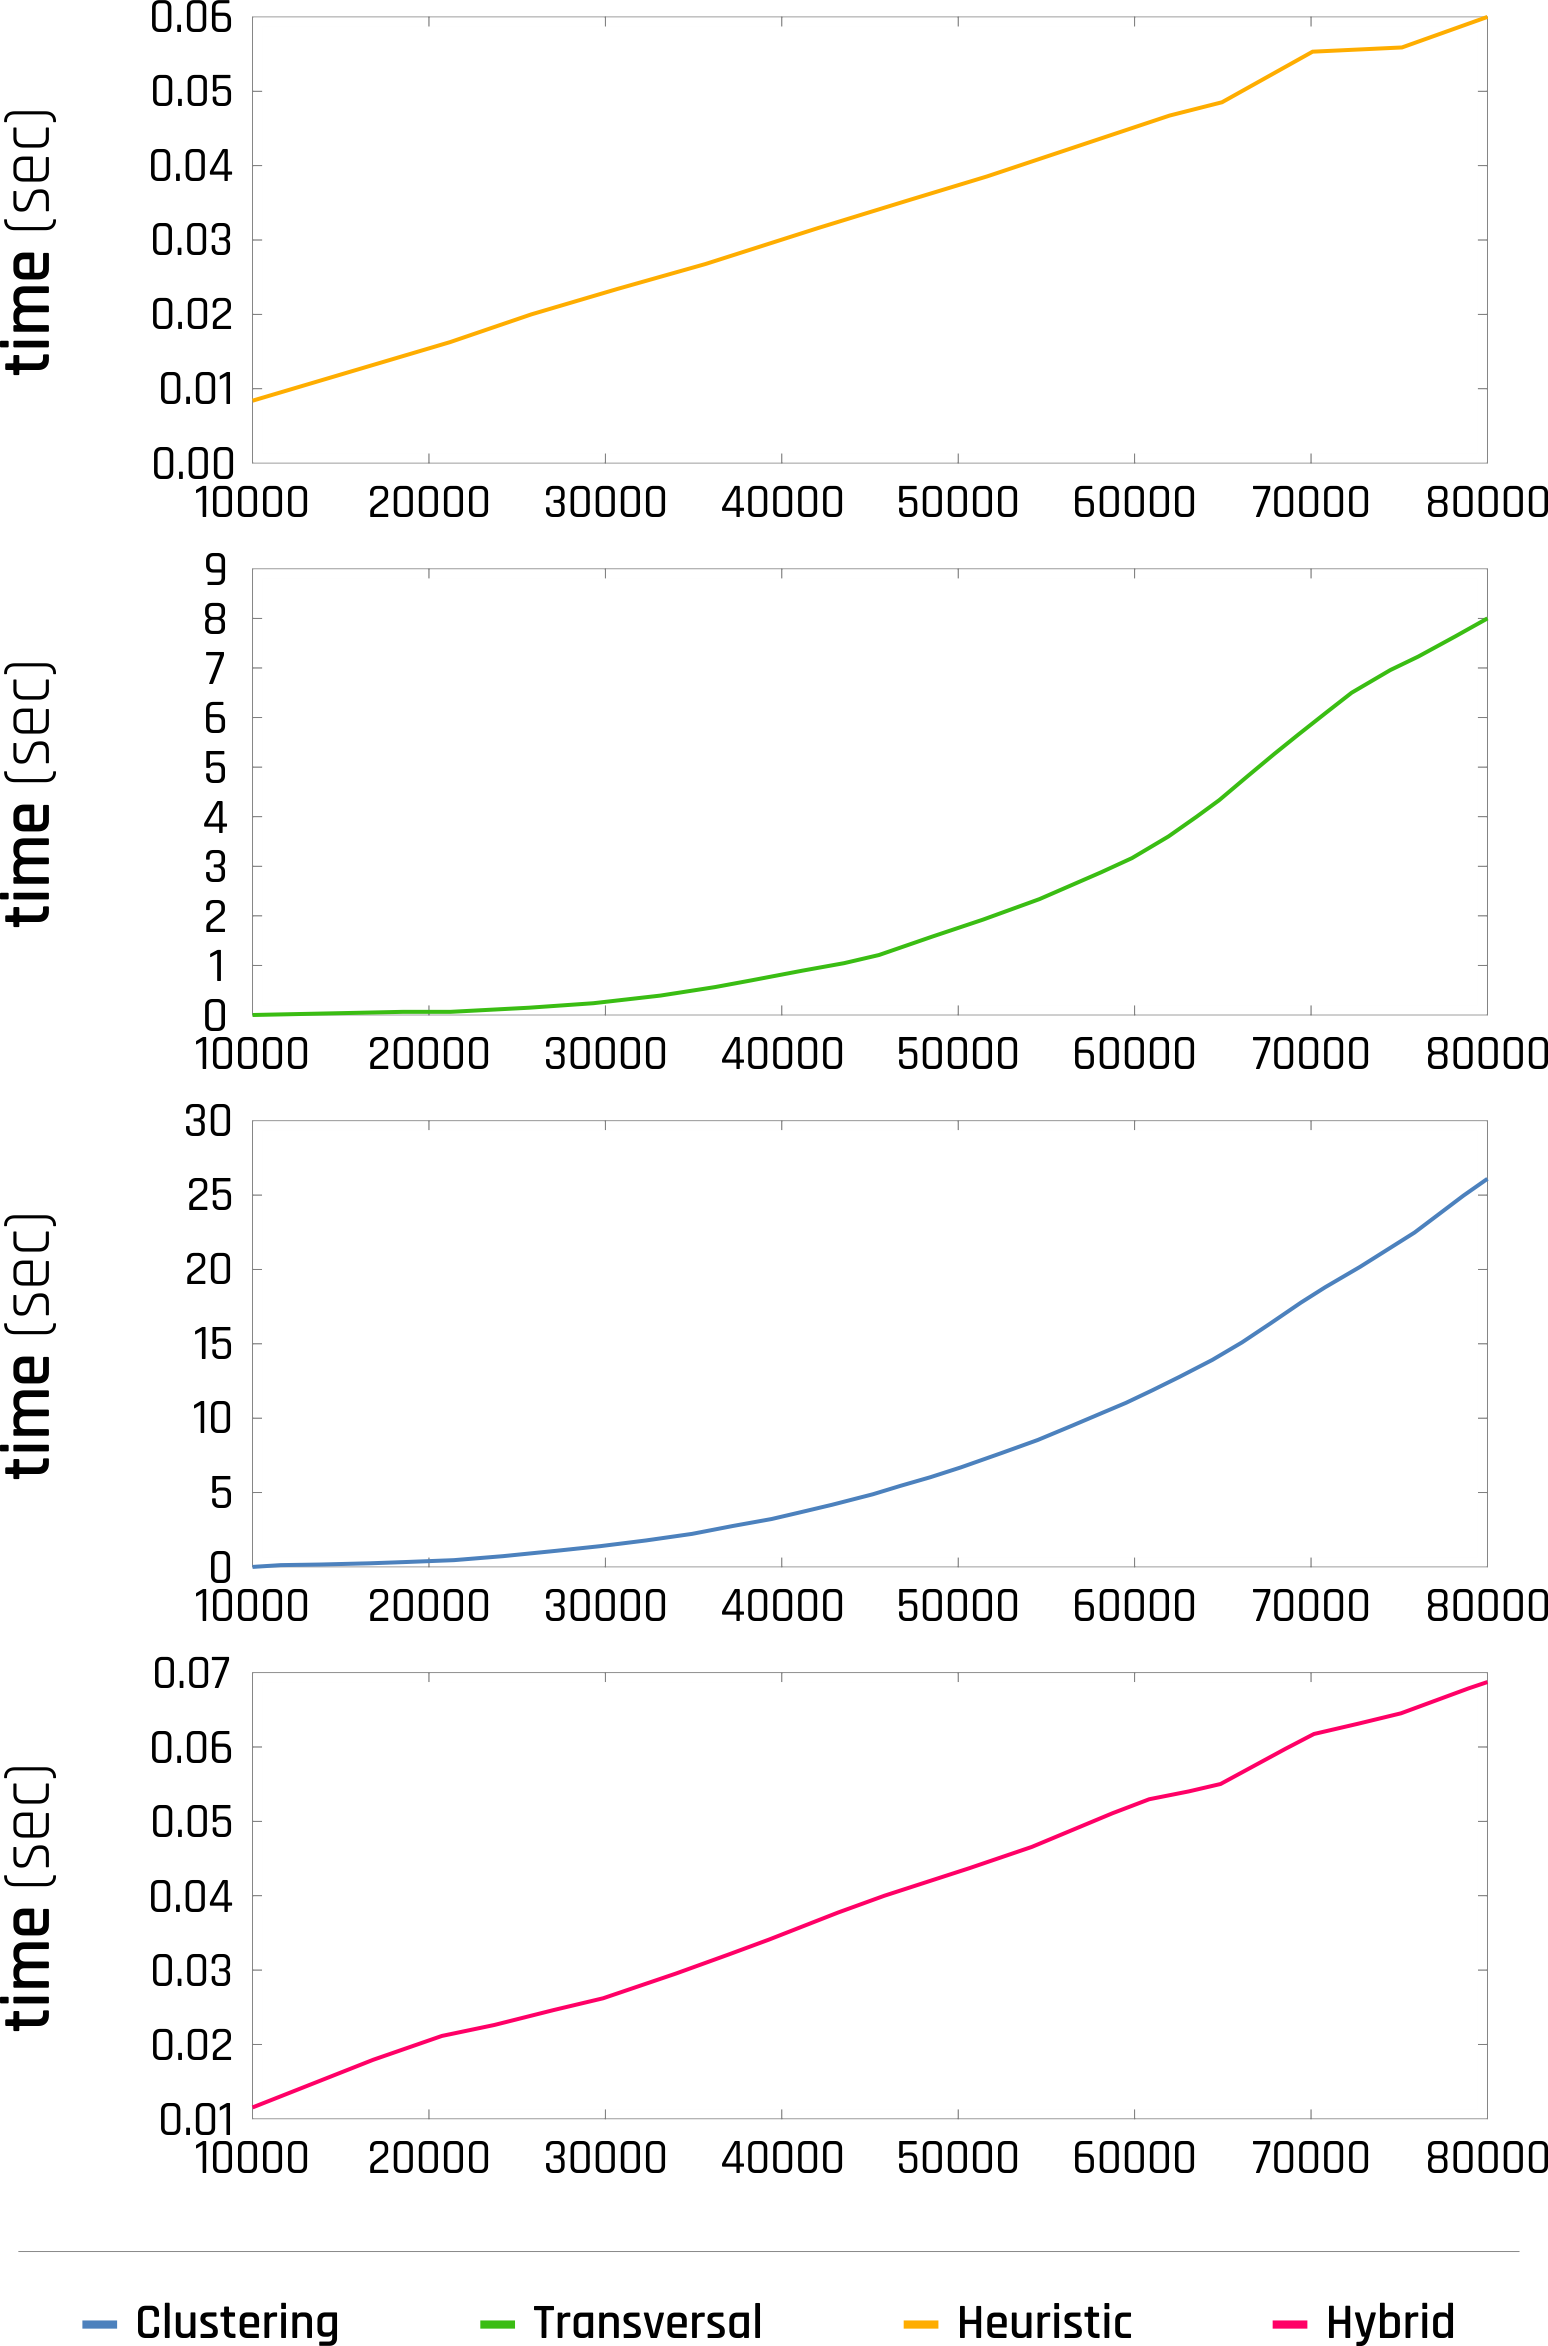
\includegraphics[scale=1]{node_scaling.png}
		\caption{Scaling against an increasing
			\newline EV population\label{fig:popscale}}
\end{figure}
\begin{figure}
		\centering
		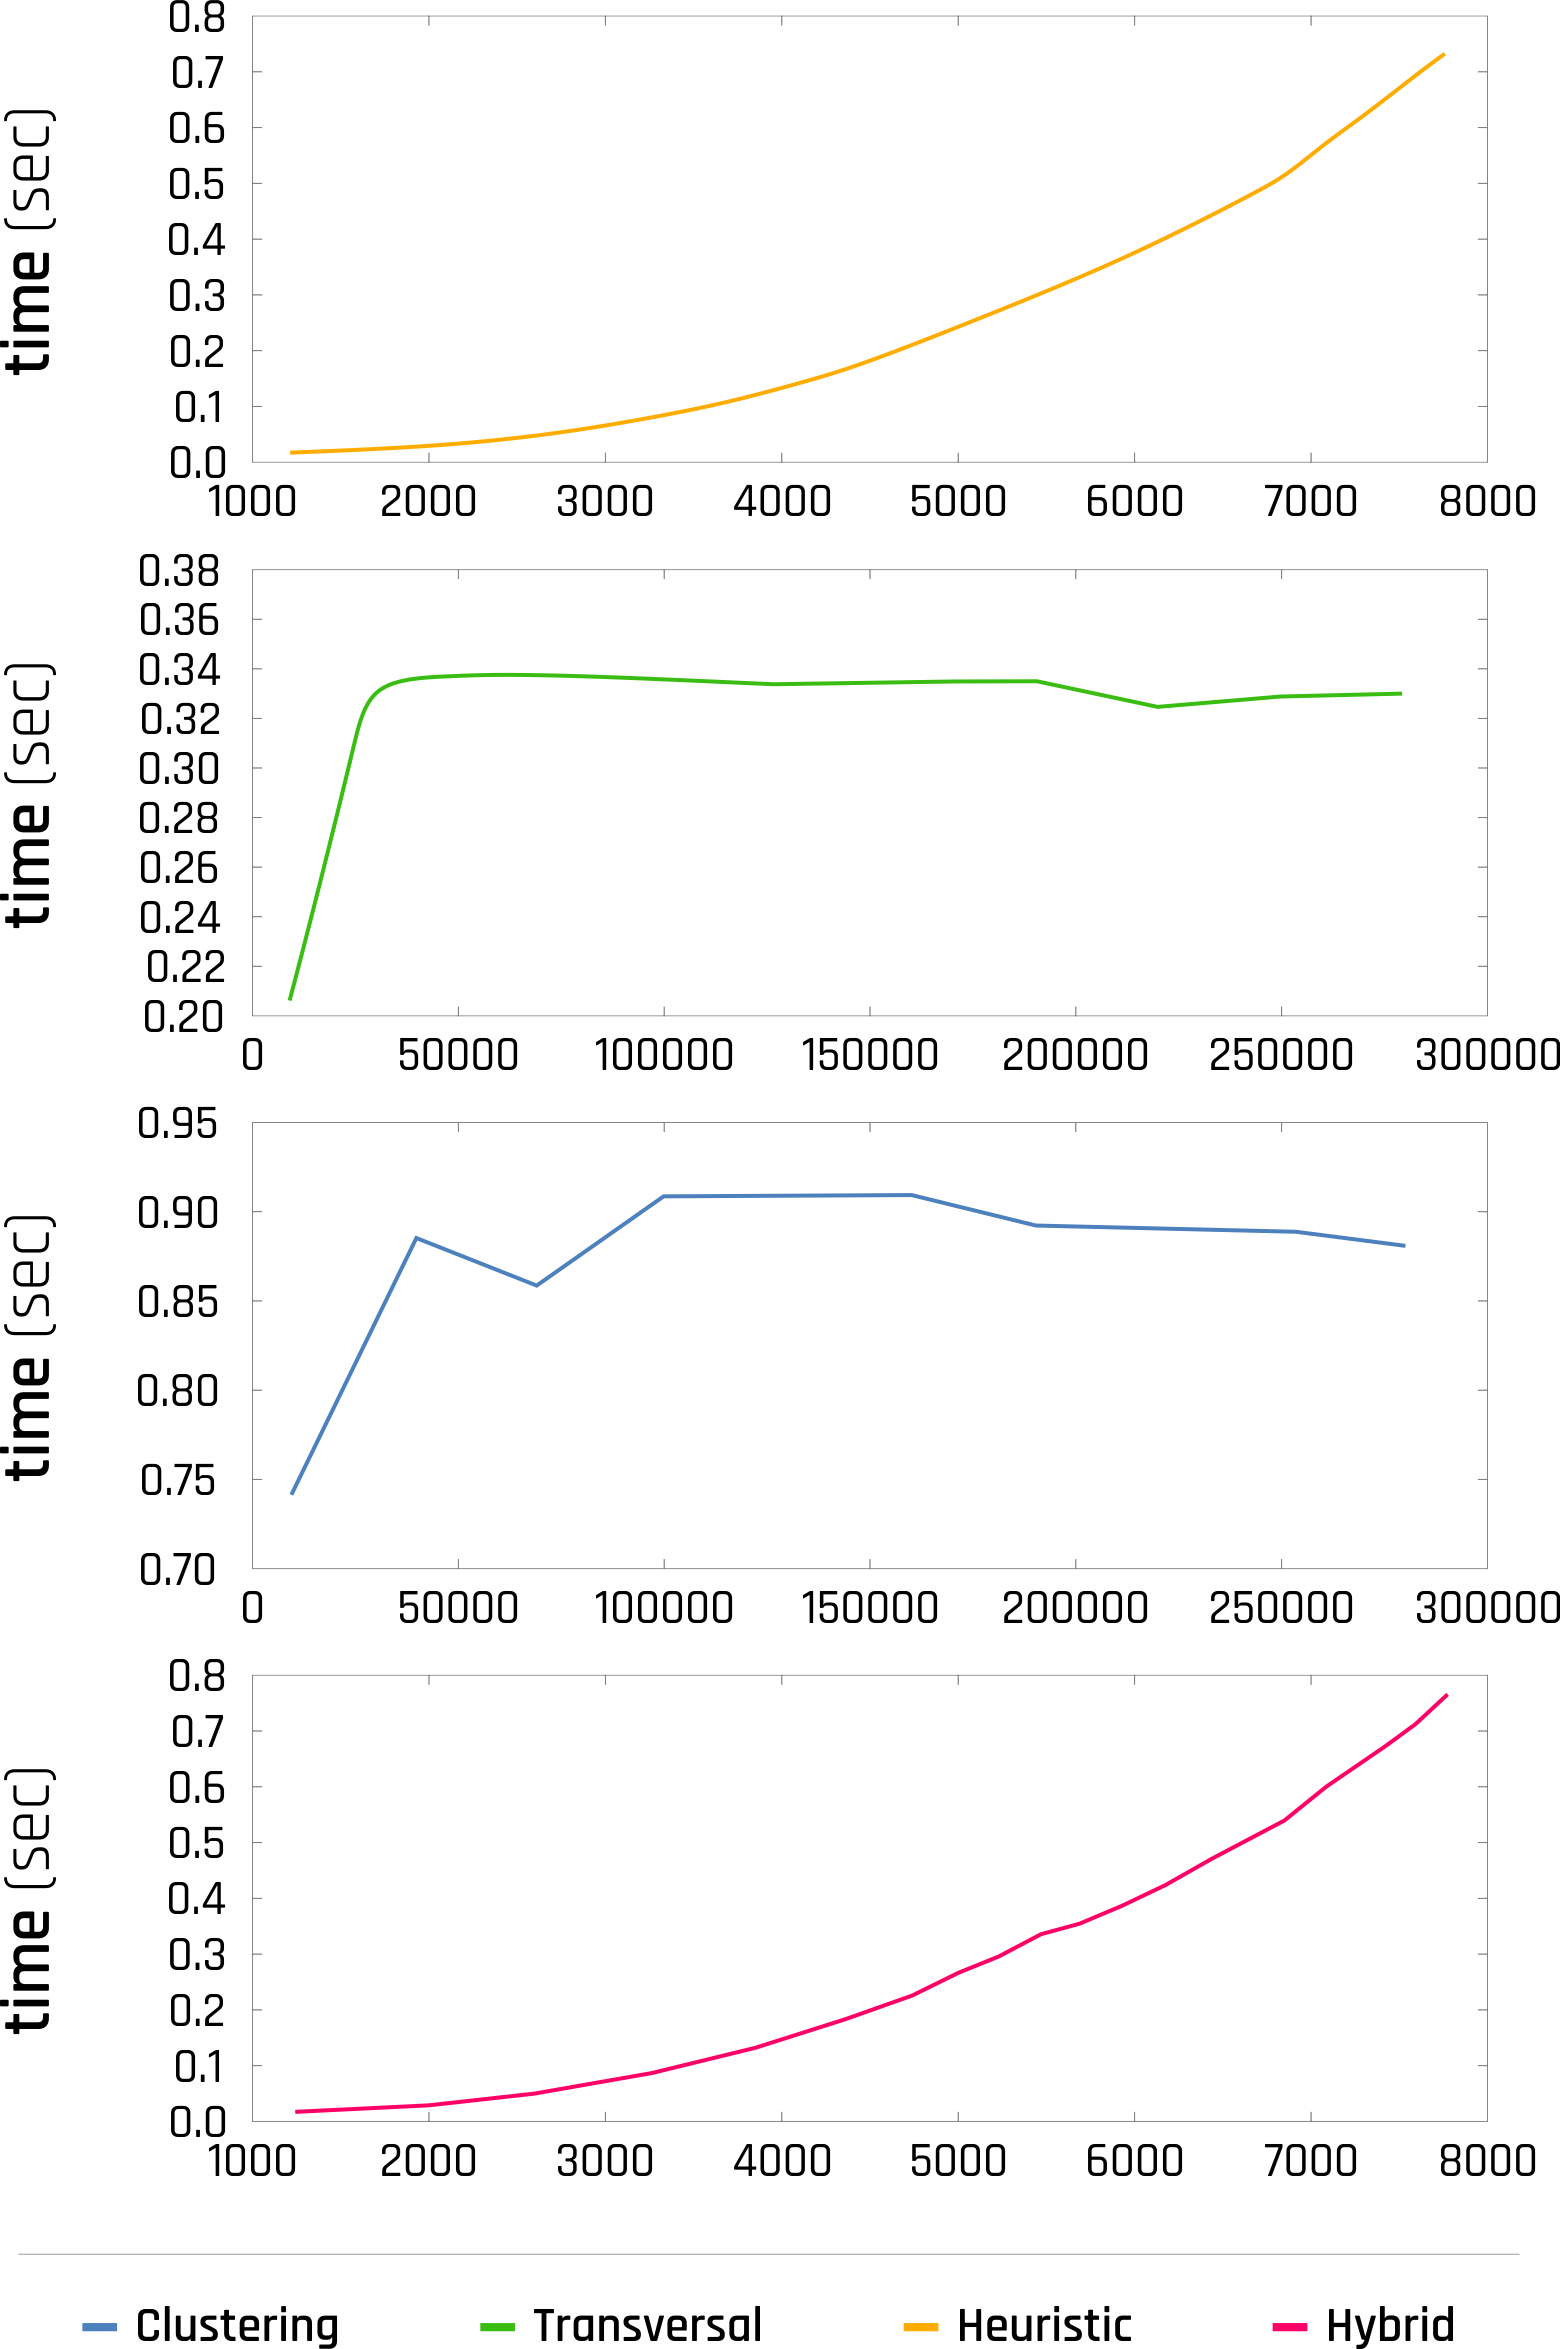
\includegraphics[scale=1]{goal_scaling.png}
		\caption{Scaling against an increasing\newline ``capacity'' goal\label{fig:goalscale}}
\end{figure}
The transversal algorithm scales with steps. The main reason for this is that the minimal transversal sets are generated before we select the agents of a coalition. If a minimal transversal set does not achieve the goal capacity, we generate a new one with more agents, till we reach the set capacity goal. This generates a step pattern, the first stages of which are shown in Fig.~\ref{fig:goalscale}. In Fig.~\ref{fig:goalscale} we actually manage to see only one step because generating the minimal transversals with $3$ EVs is enough to find good coalitions for all goals from $40,000$ $kWh$ onwards (while it was enough to generate the minimal transversals with $2$ EVs to cover the $10,000$ $kWh$ capacity goal). %Note that though it takes the transversal algorithm more than twice the time of the heuristic to scale to 300MWh, this time, is still low ($<30$sec).  
%Finally, the clustering algorithm's running time is constant irrespective of increase in the capacity goal. 
%The reason for this is that clustering, which is the part of the algorithm that requires the most processing power, takes place regardless of the final coalition requirements.
%In conclusion, the transversal algorithm exhibits the worst scaling behaviour against an increasing capacity goal, while the clustering algorithm's running time is not influenced by such an increase. 

Now, the running time of the hypegraph clustering algorithm is largely independent of the size of the stated capacity goal. 
This is because the clustering itself, which is the part of the algorithm that requires the most processing power, takes place regardless of the final coalition requirements.
Indeed, we observe in Fig.~\ref{fig:goalscale} that after an initial jump due to increased sampling requirements (cf. lines 6---8, Alg.~\ref{alg:clustering}) when moving from a goal of $10,000$ to $40,000$ $kWh$,
the algorithm's running time remains largely unaltered.
\begin{figure}
	\centering
	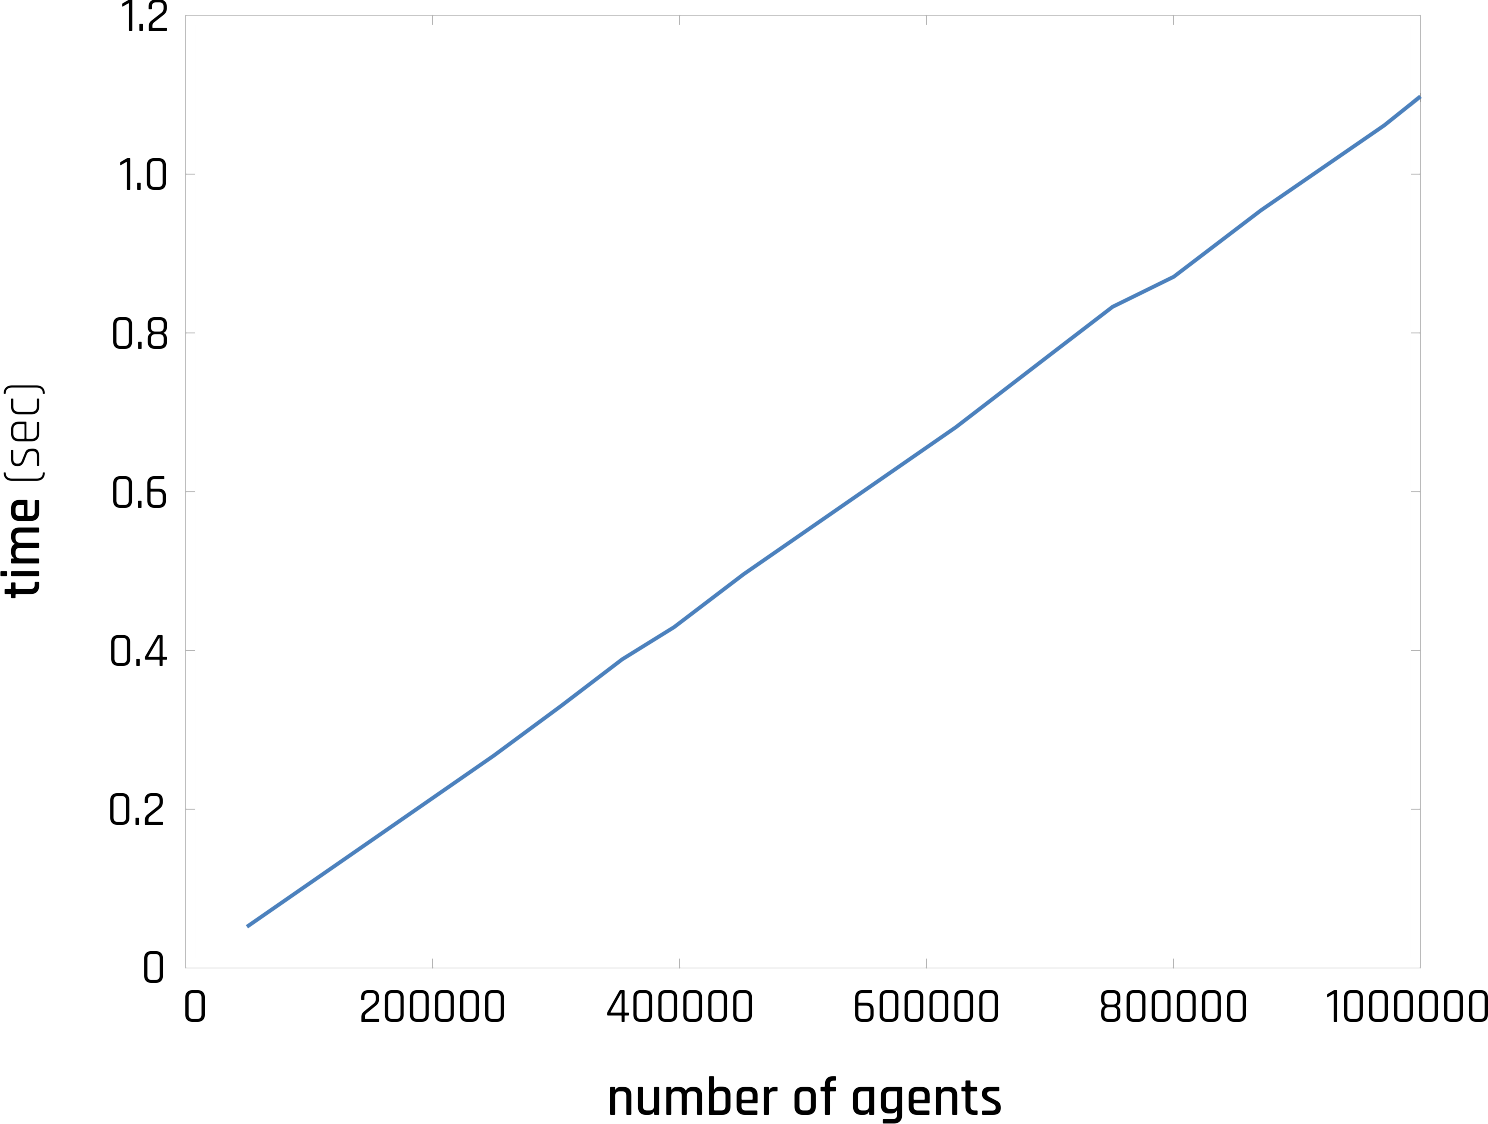
\includegraphics[scale=1]{greedy_node_scaling.png}
	\vspace{10pt}
	\caption{Scaling of the Heuristic Algorithm\label{fig:heuristicscaling}}
\end{figure}
Fig.~\ref{fig:popscale} %and table~\ref{tab:popscale} 
displays scaling against the initial EV population. The coalition goals were kept constant, and the same for all algorithms.
The heuristic algorithm shows a linear scaling in time as the agent size grows. Specifically, the heuristic algorithm can scale {\em up to a million agents} within an acceptable time. 
\begin{figure}
	\centering
	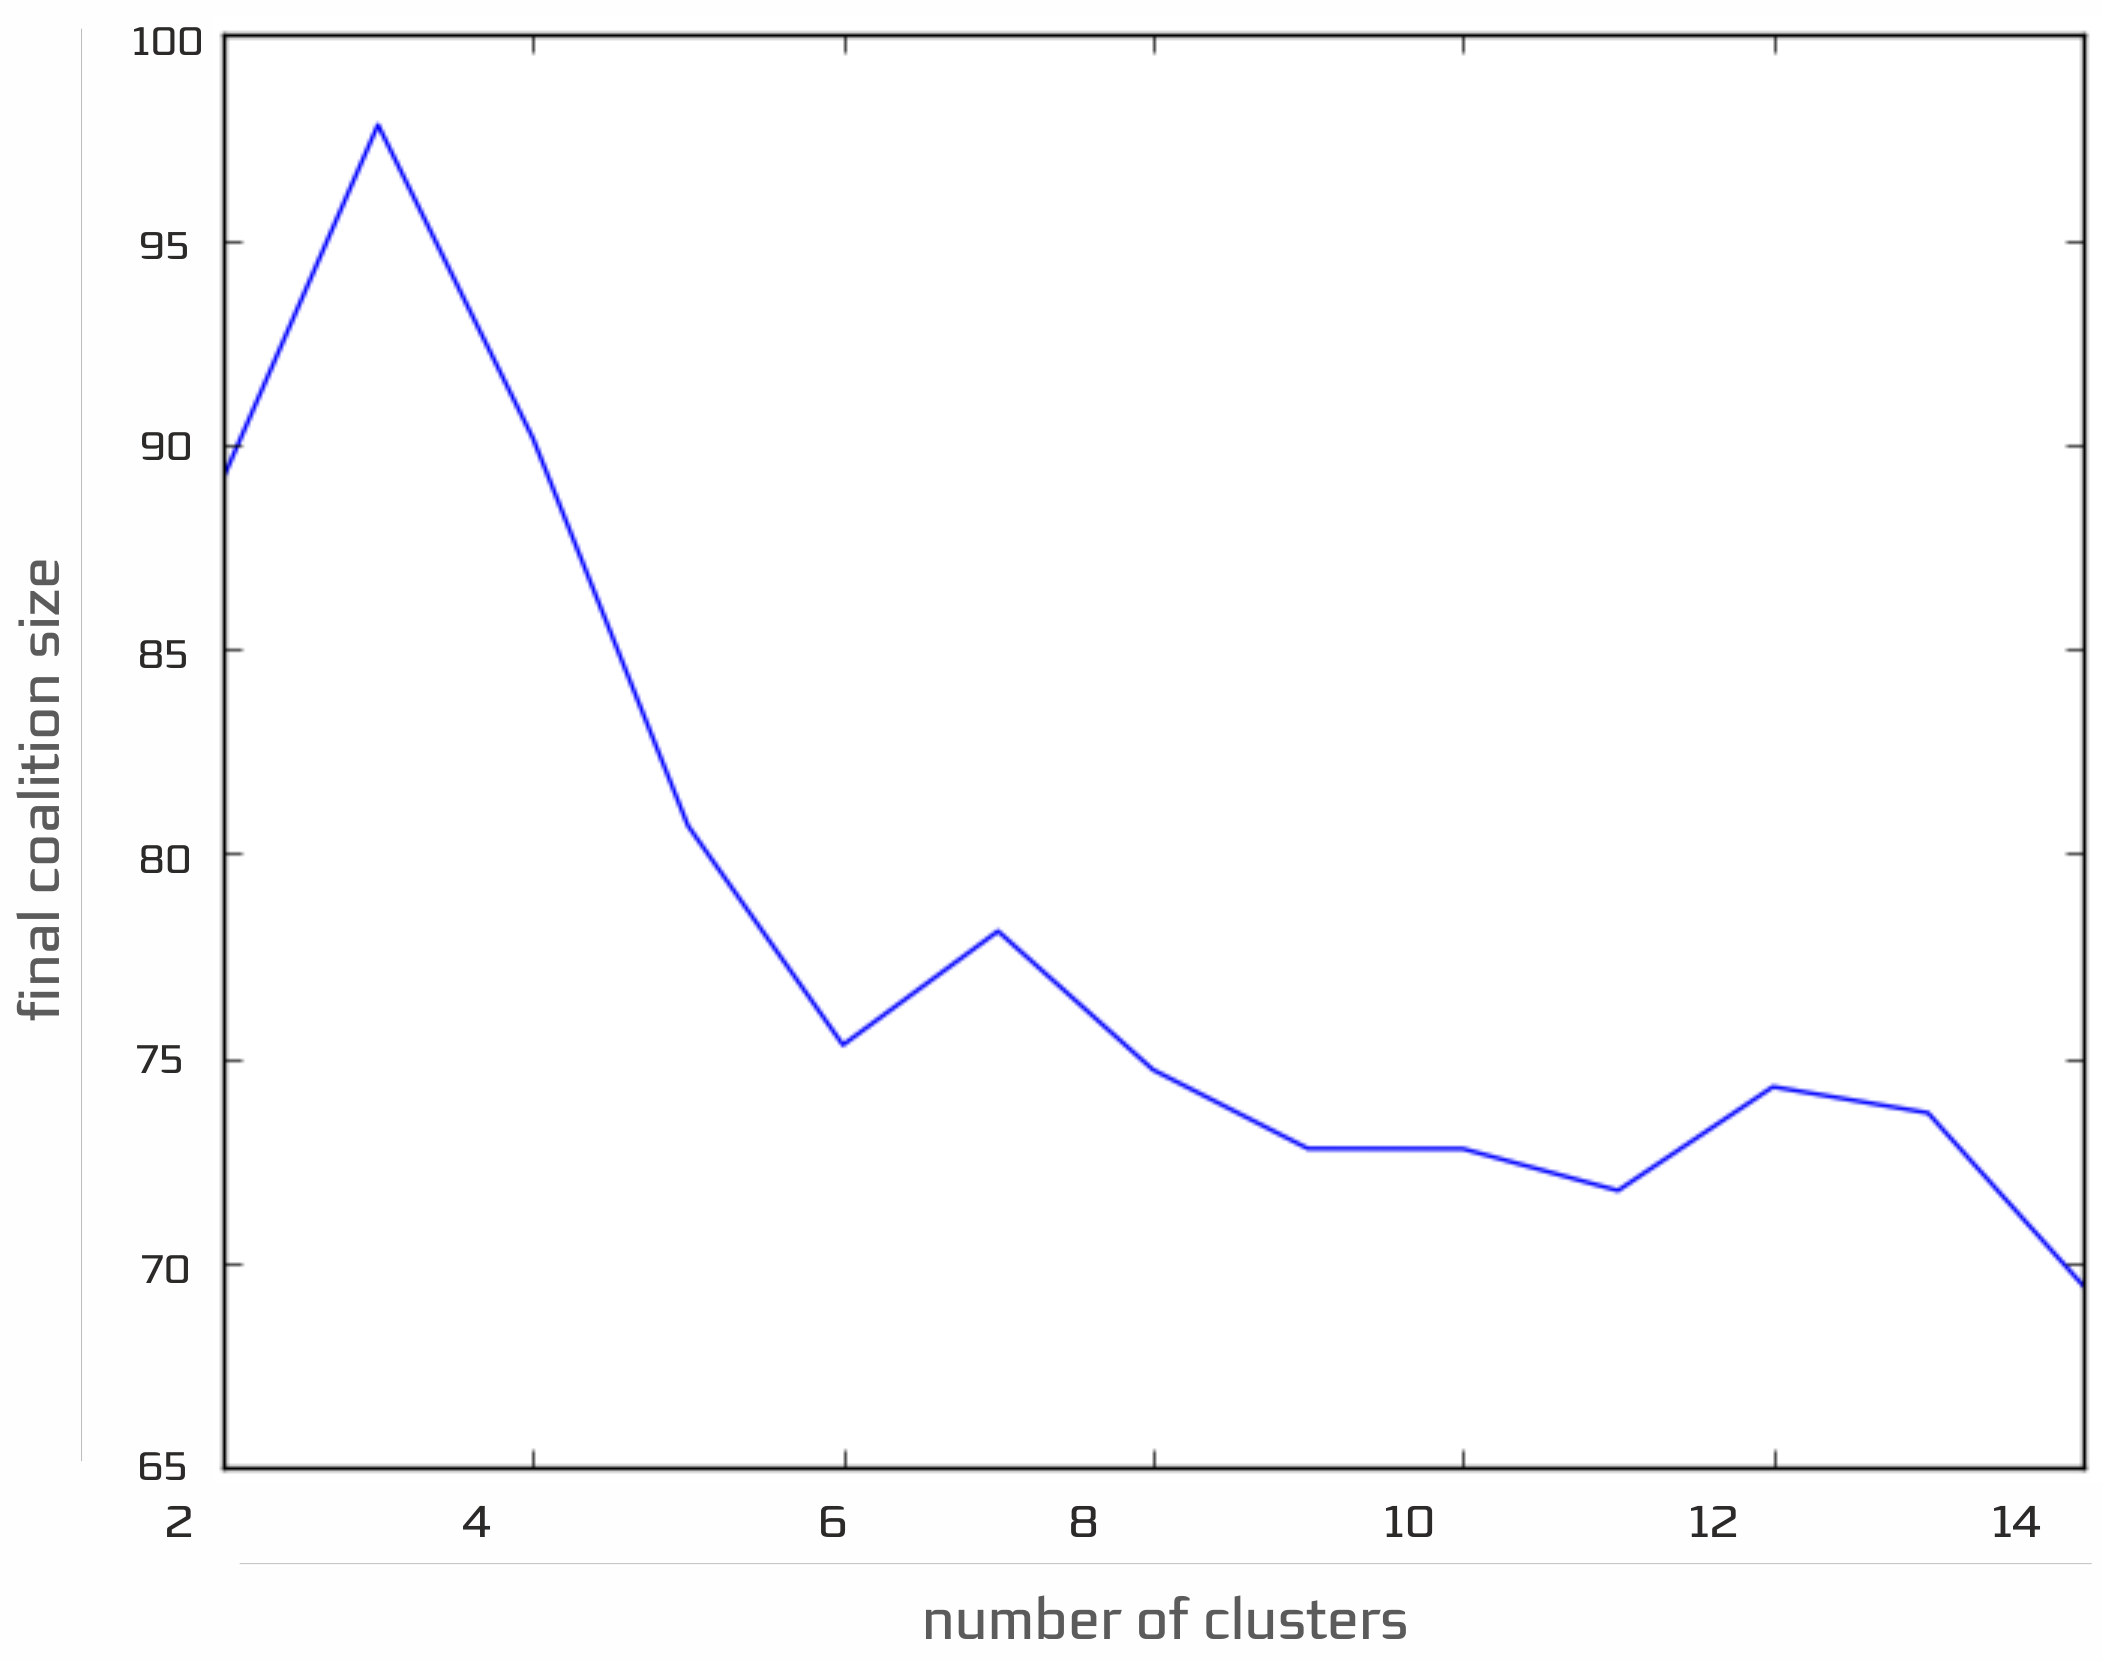
\includegraphics[scale=1]{number_of_clusters.png}
	\vspace{10pt}
	\caption{Evolution of the average size of coalitions produced with the Hypergraph Clustering method, when varying the number of clusters\label{fig:clusterkscale}}
\end{figure}

Fig.~\ref{fig:heuristicscaling} demonstrates this behaviour, starting from $50,000$ EVs. Of course, one expects that when the population reaches several millions, the complexity of the sorting algorithm will kick in, creating bottlenecks. Regardless, the fact that linear scalability is maintained up to $1,000,000$ agents is reassuring. By contrast, looking at Fig.~\ref{fig:popscale}, we observe that the transversal and clustering algorithms scale exponentially.





	\begin{table}		
		\begin{center}
			\begin{tabular}{| c || c | c | c | }
				\hline
				EVs   & Heuristic (sec) & Clustering (sec) & Transversal (sec) \\ \hline
				10,000 & 0.012 & 0.14 & 0.03  \\ \hline
				11,000 & 0.013 & 0.17 & 0.04\\ \hline
				12,000 & 0.015 & 0.22 & 0.05\\ \hline
				13,000 & 0.016 & 0.25 & 0.06  \\ \hline
				14,000 & 0.017 & 0.31 & 0.07\\ \hline
				15,000 & 0.018 & 0.11 & 0.07\\ \hline
				16,000 & 0.019 & 0.36 & 0.08 \\ \hline
				17,000 & 0.020 & 0.43 & 0.08\\ \hline
				18,000 & 0.021 & 0.50 & 0.09 \\ \hline
				19,000 & 0.023 & 0.57 & 0.10  \\ \hline
				20,000 & 0.024 & 0.69 & 0.12\\ \hline
			\end{tabular}
		\end{center}
		\caption{Scaling against an increasing EV population\label{tab:popscale}}
	\end{table}

\section{Varying the number of hypergraph clusters} \label{sec:results_modifications}
We test our clustering algorithm further by modifying the number of clusters, $k$, since this is a parameter that can be optimized empirically, as explained in Section~\ref{sec:Clustering}.

Fig.~\ref{fig:clusterkscale} displays the relation between \textit{k} and the average coalition size that results from the clustering method (and which achieves the set goals). Creating a larger number of clusters results in smaller, and thus better, coalitions. Regardless, even when $k=15$, the clustering algorithm still produces coalitions with more EVs than the heuristic one.% ($69$ compared to $58.5$).
